% !TEX root = ANA-GENR-2018-01-INT1.tex
% Turn off some chktex warnings.
% chktex-file 1 chktex-file 8 chktex-file 46

%------------------------------------------------------------------------------
\section{The FENCE project}%
\label{sec:The_FENCE_project}
%------------------------------------------------------------------------------

FENCE is an object-oriented \textit{PHP}~\cite{php} framework designed for the development of web applications. It encompasses the concepts of encapsulation, data abstraction, polymorphism and inheritance. A class can be defined as a template that describes the behaviour that the object of its type support. FENCE assembles classes to build applications by making extensive use of configuration files. Configuration files are loaded into the engine at each request to then generate the HTML response to the user’s browser.
Since it promotes reuse, similar features are implemented from predefined software components and, therefore, it speeds up the development process and reduces maintenance costs.
The FENCE software development process encompasses Software Engineering methods such as requirements analysis, architecture, design, testing, deployment and maintenance in order to guarantee the quality of the software. Requirements are gathered and documented prior to the solution design and, in this way, developers are able to propose broader solutions that can benefit the whole project. After any implementation is done, software tests are run to assure software correctness, robustness, extensibility and reusability. Currently, there are more than 20 ATLAS web systems in production that were developed using the FENCE framework, which facilitates their maintenance and enhancements.

%------------------------------------------------------------------------------
\subsection{FENCE main classes}%
\label{sec:FENCE_main_classes}

The FENCE framework is composed by a library of helper classes that are extensible program-code templates for creating objects, providing initial values and implementations of functions or methods.
Any new class can be coded and added to the framework, enlarging its scope, to then be reused in different systems.
One example is the \Class{Search} class that provides methods to create search interfaces by adding only some lines of code and the specification of the search and results attributes through a configuration file.
The \Class{SuperSearch} class offers an advanced search interface, where the user can build logic queries with AND and OR operators.
The \Class{User} class supports the access control of the interfaces.
The \Class{Mailer} class can be used to send automatic emails.
Form inputs can be easily added using classes like \Class{TextInput}, \Class{DateInput} or \Class{MemberInput}, which provides a selection box with the list of all members of an experiment.

The FENCE \Class{Workflow} class is another feature that can be inherited by the systems that are implemented using the framework.
It can be applied to codify any process involving states and actions triggered while moving from a state to another.
This is used extensively by the ATLAS analysis systems, which are organised in phases, each one divided into several steps.
Each of those steps can record metadata in the ATLAS database, trigger an egroup~\cite{egroups} creation or update, an update on GitLab~\cite{gitlab}, send automatic emails and other tasks.


%------------------------------------------------------------------------------
\subsection{Configuration files in FENCE}%
\label{sec:Configuration_files_in_FENCE}

The FENCE framework proposal is based on configuration files that provide the necessary parameters and properties to build interfaces.
The main goal of this infrastructure is to simplify many aspects of web systems requirements. The configuration files are in JSON (JavaScript Object Notation), a lightweight format for storing and transporting data, and since those can be transformed in structured objects, developers can easily define a group of properties within specific contexts.
For instance, it is possible to set up which groups of users can have access to a certain interface.
Another benefit of using configuration files is that major classes, that have several arguments and environment parameters, can be instantiated in a cleaner way, with just a configuration file path as argument.
With that, developers feel encouraged to develop more generic and robust features, since they can be easily reused it in the future.

Along with the configuration file concept, additional utilities were developed to guarantee the feasibility of this idea.
\GSnote{One of these tools is the class \Class{JReader}, which parses a JSON input file, validates it and provides the JSON data to PHP code.}{How is this different from JSON Schema validation? I have a hard time understanding what it does better or different.}
\GOnote{}{I have read the documentation of JSON Schema validation and am not sure about how different it is from this class. Do you consider it better for us to ommit this class? Nonetheless, here it is a description of how JReader works: a JSON file is passed as an argument to the constructor of the class. An abstract method 'validate' has to be defined and works similarly to a JSON schema. With that, JSON is parsed and validated, but also, constants are replaced according to environment variables or methods.}
Another one is the FENCE \Class{Content} class, which gets some default information from configuration file to handle common interface needs, such as access control, constants and rendering outline formats. 

Most of the time, when a new interface is created using FENCE, the class that generates the particular content of this page is inheriting the \Class{Content} class.
At the same time, the \Class{Content} class, which has a configuration file path as argument, uses \Class{JReader} to validate and access the JSON properties. \Cref{fig:content_uml_diagram} shows the UML diagram of the Content class.

\begin{figure}[htb]
    \centering
    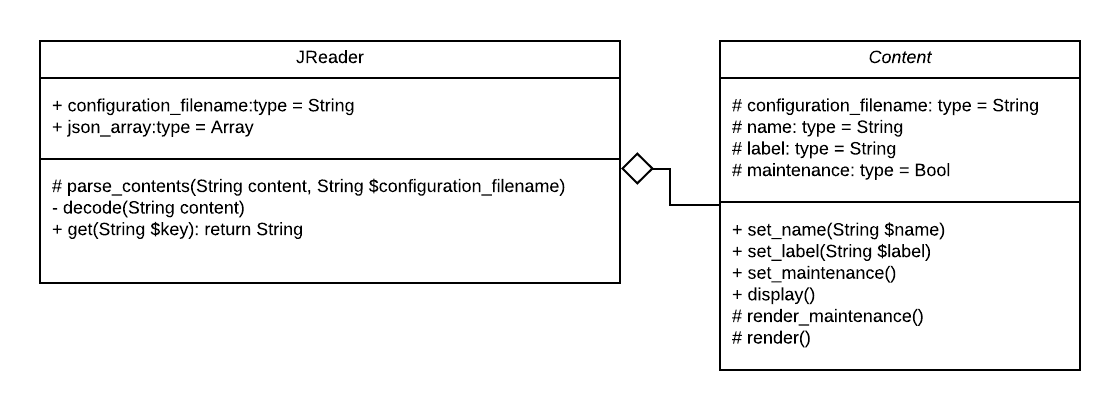
\includegraphics[width=1\textwidth]{content_uml_diagram}
    \caption{\Class{Content} class UML diagram describing its interaction with \Class{JReader}}%
    \label{fig:content_uml_diagram}
\end{figure}

\GSnote{}{Do you have a block-tree diagram that shows all of these relationships? Something like the one that gets generated when you run doxygen on C++ code}
\GOnote{}{We have included the UML diagram of Content class that way, since for an internal note it would be expected that the reader understands it. In case we turn it into a pubnote, then we will have no explain better the diagram. We found doxygen even more complicated.}